\documentclass[dvipdfmx]{jsarticle}
\usepackage{amsmath,amssymb}
\usepackage[dvipdfmx]{graphicx}
\usepackage{physics}
% table
\usepackage{booktabs}
% unit and No.
\usepackage{siunitx}
\sisetup{separate-uncertainty=true}
% calligraphy
\usepackage{bm}
\usepackage{color}
\usepackage{mathrsfs}
% hyperlink
\usepackage{hyperref}
\usepackage{pxjahyper}
% displaying codes
\usepackage{listings}
% page rotation
\usepackage{lscape}
% subcaption of fig.
\usepackage{subcaption}
% tikz
\usepackage{tikz}
\usepackage{circuitikz}
\usetikzlibrary{intersections,calc,arrows.meta}
\usetikzlibrary{circuits.logic.US}
\usetikzlibrary{positioning, fit}
% for writing codes
\lstnewenvironment{mylisting}[1][]
    {\lstset{
        breaklines=true,
        frame=single,
        basicstyle=\ttfamily,
        numbers=left,
        numbersep=10pt,
        tabsize=4,
        extendedchars=true,
        xleftmargin=24pt,
        framexleftmargin=24pt,
        #1
    }
}{}
% no page no.
\pagestyle{empty}

\title{宇宙線観察から学ぶ粒子の崩壊とスピン回転
}

\begin{document}
\maketitle

\section{理論}

\subsection{ミュオンの生成}
\label{sec: theory: generation of muon}

ミュオン$\mu^-$は第2世代の荷電レプトンであり, 地表に到達する2次宇宙線の大部分を占め, 荷電粒子のおよそ80\%である\cite{Grupen}.
水平面積$\SI{1}{\cm^2}$に$\SI{1}{\min}$あたりおよそ$1$個のミュオンが平均$\SI{4}{\GeV}$で飛来する\cite{PDG}.
電荷は$-1$, スピン$1/2$, 質量$\SI{105.6583745\pm0.0000024}{\MeV}$で電子の約200倍あり, 平均寿命は$\SI{2.1969811\pm0.0000022}{\micro\second}$である\cite{PDG}.
2次宇宙線のミュオンは主に荷電パイオンの崩壊によって生じる.
1次宇宙線の陽子が大気上層で
\begin{align*}
    &p+p\to p+n+\pi^+
    \\
    &p+n\to p+p+\pi^-
    \\
    &p+n\to p+n+\pi^++\pi^-
\end{align*}
の反応を起こしてパイオンが生じ,
\begin{align*}
    &\pi^+\to\mu^++\nu_\mu
    \\
    &\pi^-\to\mu^-+\bar{\nu}_\mu
\end{align*}
と崩壊する.

ニュートリノのヘリシティは負のみ, 反ニュートリノは正のみであるから, 角運動量保存よりパイオン静止系にて$\mu^+$のスピンは運動量と同じであり, $\mu^-$は逆となる(図\ref{fig: pion decay}).
パイオンの崩壊は主に電磁シャワー内部で生じることを考慮すると, 図\ref{fig: muon shower}のように実験室系にて地表に降り注ぐ向きの運動量が大きい$\mu^+$はスピンが上向き, $\mu^-$はスピンが下向きになる割合が多くなると考えられる.
% 定量的なことを言いたい

\begin{figure}
    \centering
    \begin{tabular}{cc}
        \begin{minipage}[t]{0.3\hsize}
            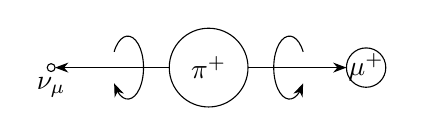
\begin{tikzpicture}
    \coordinate(pi)at(0,0);
    \coordinate(mu)at(2,0);
    \coordinate(nu)at(-2,0);
    \draw
        (pi)circle[radius=.5]node[anchor=center]{$\pi^+$}
        (mu)circle[radius=.25]node[anchor=center]{$\mu^+$}
        (nu)circle[radius=.05]node[anchor=north]{$\nu_\mu$}
    ;
    \draw[-Stealth]($(pi)+(.5,0)$)--($(mu)+(-.25,0)$);
    \draw[-Stealth]($(pi)+(-.5,0)$)--($(nu)+(.05,0)$);
    \draw[-Stealth]($(pi)+(-1.2,.2)$)arc(150:-150:.2 and .4);
    \draw[-Stealth]($(pi)+(1.2,.2)$)arc(30:330:.2 and .4);
\end{tikzpicture}

            \caption{$\pi^+$の崩壊}
            \label{fig: pion decay}
        \end{minipage}
        &
        \begin{minipage}[t]{0.4\hsize}
            \centering
            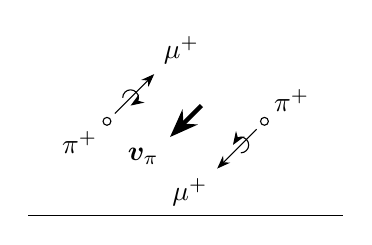
\begin{tikzpicture}
    \coordinate(O)at(0,.8);
    \coordinate(pi1)at(1,2);
    \coordinate(pi2)at(3,2);
    \draw(O)--++(4,0);
    \draw(pi1)circle[radius=.05]node[anchor=north east]{$\pi^+$};
    \draw(pi2)circle[radius=.05]node[anchor=south west]{$\pi^+$};
    \draw[-Stealth]($(pi1)+(.1,.1)$)--++(.5,.5)node[anchor=south west]{$\mu^+$};
    \draw[Stealth-]($(pi1)+(.3,.3)+(.0,-.1)$)arc(-90:180:.1);
    \draw[-Stealth]($(pi2)+(-.1,-.1)$)--++(-.5,-.5)node[anchor=north east]{$\mu^+$};
    \draw[-Stealth]($(pi2)+(-.3,-.3)+(.0,-.1)$)arc(-90:180:.1);
    \draw[ultra thick,-Stealth]($(pi1)!.5!(pi2)+(.2,.2)$)--++(-.4,-.4)
    node[anchor=north east]{$\bm{v}_\pi$};
\end{tikzpicture}

            \caption{地表に降り注ぐ荷電粒子とスピン}
            \label{fig: muon shower}
        \end{minipage}
    \end{tabular}
\end{figure}


\subsection{ミュオンの崩壊}
\label{sec: theory: decay of muon}

宇宙線ミュオンは地表に降り注ぐ間は固有時間がほとんど進まないが,
\footnote{
    高度$\SI{15}{\km}$にて生成し地表での平均エネルギー$\SI{4}{\GeV}$で飛来する間のミュオンの固有時間は〜と概算される.
    これに加えて空中で$\SI{2}{\GeV}$減衰することを考慮すると, 固有時間は寿命に比べて十分短い.
    数値は全て\cite{PDG}より.
}
資料にトラップされると平均寿命$\SI{2.2}{\micro\second}$で崩壊し電子または陽電子を放出する.
\begin{align*}
    &\mu^+\to e^++\nu_e+\bar{\nu}_\mu
    \\
    &\mu^-\to e^-+\bar{\nu}_e+\nu_\mu
\end{align*}
エネルギーとスピンに依存する(陽)電子の放出方向の分布は定数係数を除いて以下の式で近似される\cite{PDG}.
\begin{equation*}
    \frac{\dd[2]{\Gamma}}{\dd{x}\dd{\cos\theta}}
    \propto
    [3-2x\pm P_\mu\cos\theta(2x-1)]x^2
\end{equation*}
ただし$x=2E_e/\mu$で, $\theta$は電子の運動量とミュオンのスピンの間の角である.
簡単な場合に図示すると図\ref{fig: muon decay distrib.}のようになる.
すなわち, $\mu^+$はスピンと同じ向きに陽電子を, $\mu^-$はスピンと逆向きに電子を出しやすい.

\begin{figure}
    \centering
    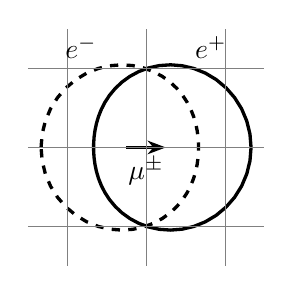
\begin{tikzpicture}
    \draw
        [very thick,samples=50,domain=0:2*pi,variable=\theta]plot(\theta/pi*180:{1+cos(\theta/pi*180)/3})
    ;
    \draw
        [dashed, very thick,samples=50,domain=0:2*pi,variable=\theta]plot(180-\theta/pi*180:{1+cos(\theta/pi*180)/3})
    ;
    \draw[-Stealth, thick](-.25,0)--(.25,0);
    \draw[step=1,gray,very thin](-1.5,-1.5)grid(1.5,1.5);
    \node at(-.5,1)[anchor=south east]{$e^-$};
    \node at(.5,1)[anchor=south west]{$e^+$};
    \node at(0,0)[anchor=north]{$\mu^\pm$};
\end{tikzpicture}

    \caption{$\mu^\pm$のスピン(矢印)と崩壊にて放出される$e^+$(実線)及び$e^+$(破線)の分布}
    \label{fig: muon decay distrib.}
\end{figure}

\ref{sec: theory: generation of muon}を合わせて踏まえると, 地表に降り注ぐミュオンのうち運動量の大きいものは上向きに, 運動量の小さいものは下向きに(陽)電子を多く放出する.


\subsection{負ミュオンの原子核捕獲}
\label{sec: theory: negative muon capture}

一部の$\mu^-$は物質中に侵入すると原子核のCoulombポテンシャルにとらわれミュオン原子を形成する.
この$\mu^-$は特性X線やオージェ電子を放出して次第に低準位へ遷移し, やがて原子核へ落ち込む.
原子核にて陽子と弱い相互作用をすることで中性子を放出する.
\begin{equation*}
    \mu^-+p\to n+\nu_\mu
\end{equation*}

(陽)電子だけでなく中性子も検出する装置を使うと, $\mu^-$の減衰比には通常の崩壊に加えてこの原子核捕獲の確率も加わるため, 見かけの寿命は$\mu^+$に比べて短くなる.
寿命変化は原子核に依存し, 今回使用した試料に含まれる元素では表\ref{table: theory: life of muon}のようになる\cite{Ito Kaji Tabata Yoshiwara}.

% もうちょい桁数ほしい
\begin{table}
    \centering
    \caption{各元素における$\mu^-$の寿命変化}
    \begin{tabular}{lrr}
        \toprule
        元素 & 文献値$[\unit{\micro\second}]$
        \\
        \midrule
        Cu & 0.16
        \\
        Al & 0.86
        \\
        Ca & 0.33
        \\
        C & 2.04
        \\
        O & 0.81
        \\
        \bottomrule
    \end{tabular}
    \label{table: theory: life of muon}
\end{table}

% 元素を混ぜた時の寿命についても書きたい

ミュオンが試料に停止してから崩壊して(陽)電子を出すまでの時間$t$を計測し, $(t,t+\Delta t)$のカウント$N(t)$をヒストグラムで集計すれば, $\mu^-$の寿命変化及び計測のバックグラウンド$BG$を反映して以下の式が成立すると考えられる.
\begin{equation}
    \label{eq: N of t considering different tau and BG}
    N(t)
    =
    N_0^+e^{-t/\tau_+}
    +
    N_0^-e^{-t/\tau_-}
    +
    BG
\end{equation}


\subsection{ミュオンのスピン偏極検出}

\ref{sec: theory: decay of muon}に基づけば, 運動量の比較的大きいミュオンが多くトラップされるとき, 試料を上下2つの検出器で挟むと上側で(陽)電子をより多く検出する.
しかし上下の検出数の差がスピン偏極によるものなのか検出器の特性によるものなのかを判断することは難しい.
そこで偏極の検出では一般にミュオンスピン回転(µSR)と呼ばれるLarmor歳差運動を用いた方法を採る.

\begin{figure}[b]
    \centering
    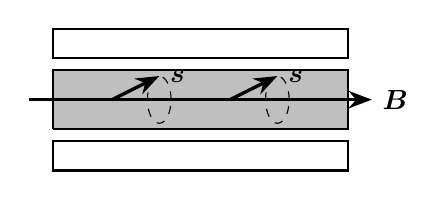
\begin{tikzpicture}[scale=1.5]
    \coordinate(Dleftdown)at(0,.25);
    \coordinate(Pleftdown)at(0,.6);
    \coordinate(Uleftdown)at(0,1.2);
    \draw[thick](Dleftdown)rectangle++(2.5,.25);
    \draw[thick](Uleftdown)rectangle++(2.5,.25);
    \filldraw[fill=lightgray, thick](Pleftdown)--++(2.5,0)--++(0,.5)--++(-2.5,0)--++(0,-.5);
    \draw[-Stealth, very thick]($(Pleftdown)+(.5,.25)$)--++(.4,.2)node[anchor=west]{$\bm{s}$};
    \draw[-Stealth, very thick]($(Pleftdown)+(1.5,.25)$)--++(.4,.2)node[anchor=west]{$\bm{s}$};
    \draw[-Stealth, very thick]($(Pleftdown)+(-.2,.25)$)--++(2.9,0)node[anchor=west]{$\bm{B}$};
    \draw[dashed]($(Pleftdown)+(.9,.25)$)circle[x radius=.1,y radius=.2];
    \draw[dashed]($(Pleftdown)+(1.9,.25)$)circle[x radius=.1,y radius=.2];
\end{tikzpicture}

    \caption{Larmor歳差運動を用いたミュオンスピン検出実験の配置. 着色部で表す試料の上下を検出器で挟む. 水平に磁場をかけるとスピンが歳差運動し, 崩壊の際に放出される粒子の分布が上下で時々刻々と変化する. }
    \label{fig: Larmor spin}
\end{figure}

図\ref{fig: Larmor spin}に示すように, 磁気回転比$\gamma$のミュオンに磁場$\bm{B}$がかかったとき,
\begin{equation}
    \label{eq: Larmor precession}
    \bm{\omega}=\gamma\bm{B}
\end{equation}
でスピンは際差運動する.
ここで$\gamma=2\pi\times\SI{135.5342}{\mega\hertz/\tesla}$である.
したがって\ref{sec: theory: decay of muon}によれば, 放出(陽)電子の角度分布も磁場を軸に回転し, 粒子の検出数が崩壊時間によって変化する(図\ref{fig: theory: N under Larmor}).

\begin{figure}
    \centering
    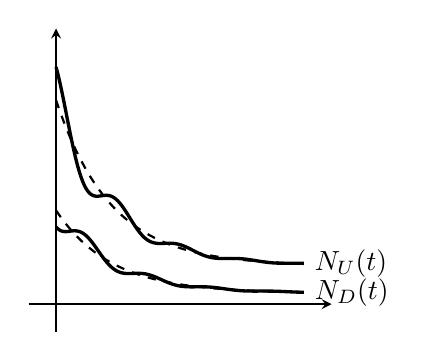
\begin{tikzpicture}[samples=200, scale=.7]
    \coordinate(O)at(0,0);
    \draw[->,>=stealth,semithick](-.5,0)--(5,0);
    \draw[->,>=stealth,semithick](0,-.5)--(0,5);
    \draw[very thick, domain=0:4.5]
    plot(\x,{3*(1+.2*cos(2*pi*50*\x))*exp(-\x)+.7})
    node[anchor=west]{$N_U(t)$}
    ;
    \draw[thick, dashed, domain=0:4.5]
    plot(\x,{3*exp(-\x)+.7})
    ;
    \draw[very thick, domain=0:4.5]
    plot(\x,{1.5*(1-.2*cos(2*pi*50*\x))*exp(-\x)+.2})
    node[anchor=west]{$N_D(t)$}
    ;
    \draw[thick, dashed, domain=0:4.5]
    plot(\x,{1.5*exp(-\x)+.2})
    ;
\end{tikzpicture}

    \caption[]{Larmor歳差運動下で予想される粒子検出数. 破線は磁場をかけない場合. }
    \label{fig: theory: N under Larmor}
\end{figure}

上下の検出器でのカウントをそれぞれ$N_U, N_D$とし, \eqref{eq: Larmor precession}の$\bm{\omega}$の大きさを$\omega$とすれば, \ref{sec: theory: negative muon capture}で述べた$\mu^-$の原子核捕獲も考慮して, 以下の式が成り立つと考えられる.
\begin{equation}
    \label{eq: N under Larmor}
    \begin{split}
        N_U(t)
        &=
        N_{U0}^+(1+P^+\cos\omega t)e^{-t/\tau_+}
        +
        N_{U0}^-(1+P^-\cos\omega t)e^{-t/\tau_-}
        +
        BG_D
        \\
        N_D(t)
        &=
        N_{D0}^+(1-P^+\cos\omega t)e^{-t/\tau_+}
        +
        N_{D0}^-(1-P^-\cos\omega t)e^{-t/\tau_-}
        +
        BG_D
    \end{split}
\end{equation}
ここで$\tau_-$は原子核捕獲のため一般に小さく, $t\gg\tau_-$にて各式の第2項は無視できる.
加えて$\mu^-$は試料に侵入すると周囲の電子との間で相互作用してスピン偏極が破れるので$N_{U0}^-,N_{D0}^-$は小さい.
% 文献ほしい
\eqref{eq: N under Larmor}各式の第2項を無視すれば, $N_U'=N_U-BG_U, N_D'=N_D-BG_D$及び実数$\alpha$を使って,
\begin{equation}
    \label{eq: asymmetry}
    \mathscr{A}
    =
    \frac{\alpha N_D'-N_U'}{\alpha N_D'+N_U'}
    =
    \frac{(\alpha N_{D0}^+-N_{U0}^+)+(\alpha N_{D0}^++N_{U0}^+)P^+\cos\omega t}{(\alpha N_{D0}^++N_{U0}^+)+(\alpha N_{D0}^+-N_{U0}^+)P^+\cos\omega t}
\end{equation}
と表される非対称度$\mathscr{A}$は, $\alpha N_{D0}^+-N_{U0}^+=0$なる$\alpha$にて角振動数$\omega$の三角関数となる.


\section{実験・解析方法}

本演習では,
\begin{itemize}
    \item ミュオンの寿命
    \item 負ミュオンの寿命変化
    \item スピン偏極
\end{itemize}
の測定を目的とする.

\subsection{寿命測定}
\label{sec: method: life}

図\ref{fig: PSc, PMT position and muon path}に示すように試料を上下からプラスチックシンチレータ(PSc)で挟み光電子増倍管(PMT)に接続する.
試料にはCu, Alの板を重ね合わせたものと, 大理石の板とを使った.
PSc+PMTは上層から順にT,U,Dとし, 各層でシンチレーション光を別々に検出できるようにする.

宇宙線及び崩壊粒子
\footnote{$\mu^-$の原子核捕獲で生じる中性子も速度が〜となってPScの検出下限〜を上回るので, これには中性子も含む. }
% 文献ほしい. 崩壊中性子の速度とPSc内部の光速
の飛程を考慮すると, 以下の事象が考えられる.
\renewcommand{\theenumi}{(\alph{enumi})}
\begin{enumerate}
    \item \label{item: pass through}粒子が試料を通過
    \item \label{item: decay into U}崩壊時に粒子を上方へ放出
    \item \label{item: decay into D}崩壊時に粒子を下方へ放出
\end{enumerate}
事象\ref{item: pass through}ではTUD全てのPSc+PMTが反応するが, 事象\ref{item: decay into U}, \ref{item: decay into D}ではまずTUが反応しDが反応しない.
その後時間を置いて粒子が崩壊すると, 事象\ref{item: decay into U}ではUが, 事象\ref{item: decay into D}ではDが反応する.

各事象を弁別するためおおよそ図\ref{fig: circuit easy}に示す論理回路を組む.
\footnote{実際に構成した論理回路は\ref{sec: logic circuit}を参照. 2種類の試料を同時に測定するため, 入出力が2系統あるのに加えて制御系統が複雑になっている. }
左端のandゲートでミュオンが試料に停止したか検出し, 停止すればゲートジェネレータを作動, 時間測定を開始する.
このゲートジェネレータが作動している間にUまたはDで信号を検出すれば, 崩壊によって粒子が放出されたものとして同図右側のandゲートで測定を止める.

Cu, Al及び及び大理石それぞれの試料で計測は$\SI{18}{\hour}, \SI{51}{\hour}$にわたって行った.

\begin{figure}
    \centering
    \begin{tabular}[]{ccc}
        \begin{minipage}[t]{0.3\hsize}
            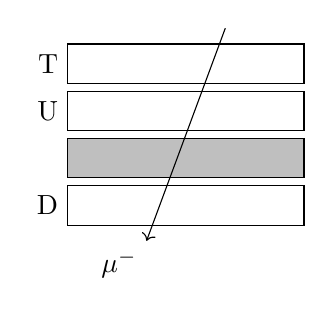
\begin{tikzpicture}
    \draw(0,0)rectangle(3,0.5);
    \fill[lightgray](0,0.6)--(0,1.1)--(3,1.1)--(3,0.6)--cycle;
    \draw(0,0.6)rectangle(3,1.1);
    \draw(0,1.2)rectangle(3,1.7);
    \draw(0,1.8)rectangle(3,2.3);
    \draw[->] (2,2.5)--(1,-0.2) node [below left]{$\mu^{-}$};
    \node [left] at (0,2.05){T};
    \node [left] at (0,1.45){U};
    \node [left] at (0,0.25){D};
\end{tikzpicture}

            \subcaption{試料を通過する場合}
        \end{minipage}
        &
        \begin{minipage}[t]{0.3\hsize}
            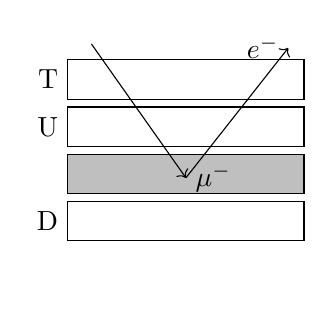
\begin{tikzpicture}
    \draw(0,0)rectangle(3,0.5);
    \fill[lightgray](0,0.6)--(0,1.1)--(3,1.1)--(3,0.6)--cycle;
    \draw(0,0.6)rectangle(3,1.1);
    \draw(0,1.2)rectangle(3,1.7);
    \draw(0,1.8)rectangle(3,2.3);
    \node [left] at (0,2.05){T};
    \node [left] at (0,1.45){U};
    \node [left] at (0,0.25){D};
    \node [below] at (1,-0.2){\textcolor{white}{$\nu_\mu$}}; %高さ調整
    \draw[->] (0.3,2.5)--(1.5,0.8) node [right]{$\mu^{-}$};
    \draw[->] (1.5,0.8)--(2.8,2.45) node [left]{$e^{-}$};
\end{tikzpicture}

            \subcaption{崩壊してUに電子を飛ばす場合}
        \end{minipage}
        &
        \begin{minipage}[t]{0.3\hsize}
            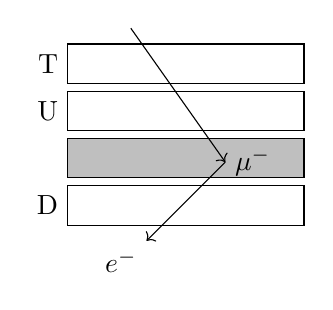
\begin{tikzpicture}
    \draw(0,0)rectangle(3,0.5);
    \fill[lightgray](0,0.6)--(0,1.1)--(3,1.1)--(3,0.6)--cycle;
    \draw(0,0.6)rectangle(3,1.1);
    \draw(0,1.2)rectangle(3,1.7);
    \draw(0,1.8)rectangle(3,2.3);
    \draw[->] (0.8,2.5)--(2,0.8) node [right]{$\mu^{-}$};
    \draw[->] (2,0.8)--(1,-0.2) node [below left]{$e^{-}$};
    \node [left] at (0,2.05){T};
    \node [left] at (0,1.45){U};
    \node [left] at (0,0.25){D};
\end{tikzpicture}

            \subcaption{崩壊してDに電子を飛ばす場合}
        \end{minipage}
    \end{tabular}
    \caption{PSc+PMTの配置と粒子の飛程. 着色部が試料を表す. }
    \label{fig: PSc, PMT position and muon path}
\end{figure}

\begin{figure}
    \centering
    \begin{circuitikz}
    \draw
    (1,0)
    % BTUnotD
    node[ieeestd and port, number inputs=3, anchor=in 1] (BTUnotD) {}
    % T
    (BTUnotD.in 1) -- ++(-1,0)
    node[anchor=east] {T}
    % GG
    (BTUnotD.out) to[short] ++(0.5,0)
    node[twoportshape, anchor=west, t=GG](GG){} ++(1,0)
    % to D stop
    -- ++(0.5,0)
    to [short, *-] ++(0,-1.5)
    -- ++(1,0)
    node[ieeestd and port, anchor=in 1] (Dstop){}
    (Dstop.out) node[anchor=west]{D stop};
    % not D
    \node at (BTUnotD.bin 3) [ocirc, left]{};
    % GG to U stop
    \draw
    (GG.east)
    to [short] ++(1.5,0)
    node[ieeestd and port, anchor=in 1](Ustop){}
    (Ustop.out) node[anchor=west]{U stop};
    \draw
    (BTUnotD.out) to[short, *-] ++(0,1)
    to[short] ++(5.2,0)
    node[anchor=west](start){start};
    \draw
    (BTUnotD.in 2) to[short] ++(-1,0)
    node[anchor=east](U){U}
    (BTUnotD.in 3) to[short] ++(-1,0)
    node[anchor=east](D){D}
    (0.5,-0.38) to [short, *-] ++(0,-1)
    -- ++(1,0)
    -| (Ustop.in 2)
    (0.7, -0.75) to [short, *-] ++(0,-1.4)
    |- (Dstop.in 2)
    ;
\end{circuitikz}

    \caption{回路の概要. GGはゲートジェネレータを表し, 入力から所定の時間(本演習では$\SI{20}{\micro\second}$)出力を続ける. }
    \label{fig: circuit easy}
\end{figure}

U, D両側で測定したカウント$N_U, N_D$を合計して, 時間を横軸としてヒストグラムにする.
% rebin 100 って何ns?
$N_U+N_D$の分布は\eqref{eq: N of t considering different tau and BG}に従うはずであるから, この式によってフィッティングし寿命$\tau_+, \tau_-$を求める.
\footnote{解析コードは\url{https://github.com/LowToneVoice/ksc16/tree/main/group7/analysis}に掲載. }


\subsection{スピン偏極測定}

\ref{sec: method: life}でのCu, Alの実験と同様にセットアップした上で, ソレノイドコイルによって水平に磁場を印加, 崩壊時間を測定する.

解析にあたっては, まず上下別々にヒストグラムを描いて
\begin{equation}
    \label{eq: method: rough fitting of spin polarization by exp}
    \begin{split}
        &N_U(t)=N_U^0e^{-t/\tau_U}+BG_U
        \\
        &N_D(t)=N_D^0e^{-t/\tau_D}+BG_D
    \end{split}
\end{equation}
でフィッティングする.
得られたバックグラウンドを除いて$N_U'=N_U-BG_U, N_D'=N_D-BG_D$とし, $\alpha$を$0.01$ずつ変えて非対称度\eqref{eq: asymmetry}を計算する.
ただし時間原点を揃える必要があるため, 回路に組み込んだ遅延を考慮して,
\begin{equation}
    \label{eq: method: fit asymmetry}
    \mathscr{A}(\alpha,t_{\text{offset}})
    =
    \frac{\alpha N_D'(t+t_{\text{offset}})-N_U'(t)}{\alpha N_D'(t+t_{\text{offset}})+N_U'(t)}
    ,
    \qquad
    t_{\text{offset}}=-\SI{30}{\nano\second}
\end{equation}
の$A\cos(2\pi ft)$によるフィッティングが最適なものを探す.
フィッティングの$\chi^2$が最小になる$\alpha$における$f$を振動数の測定値とする.

検証のため測定値$f$と\eqref{eq: Larmor precession}から磁場の強さ$B$を逆算して, ソレノイドコイルの設計上期待される値$B_\text{design}=\SI{2}{\milli\tesla}$と比較する.


\section{結果・考察}

\subsection{ミュオンの寿命}

測定データを図\ref{fig: result: CaCO3}に掲げる.
フィッティングした曲線に基づき, それぞれの試料におけるミュオンの寿命は表\ref{table: result: life}のとおりになる.

\begin{figure}
    \centering
    \begin{tabular}{cc}
        \begin{minipage}[t]{0.5\hsize}
            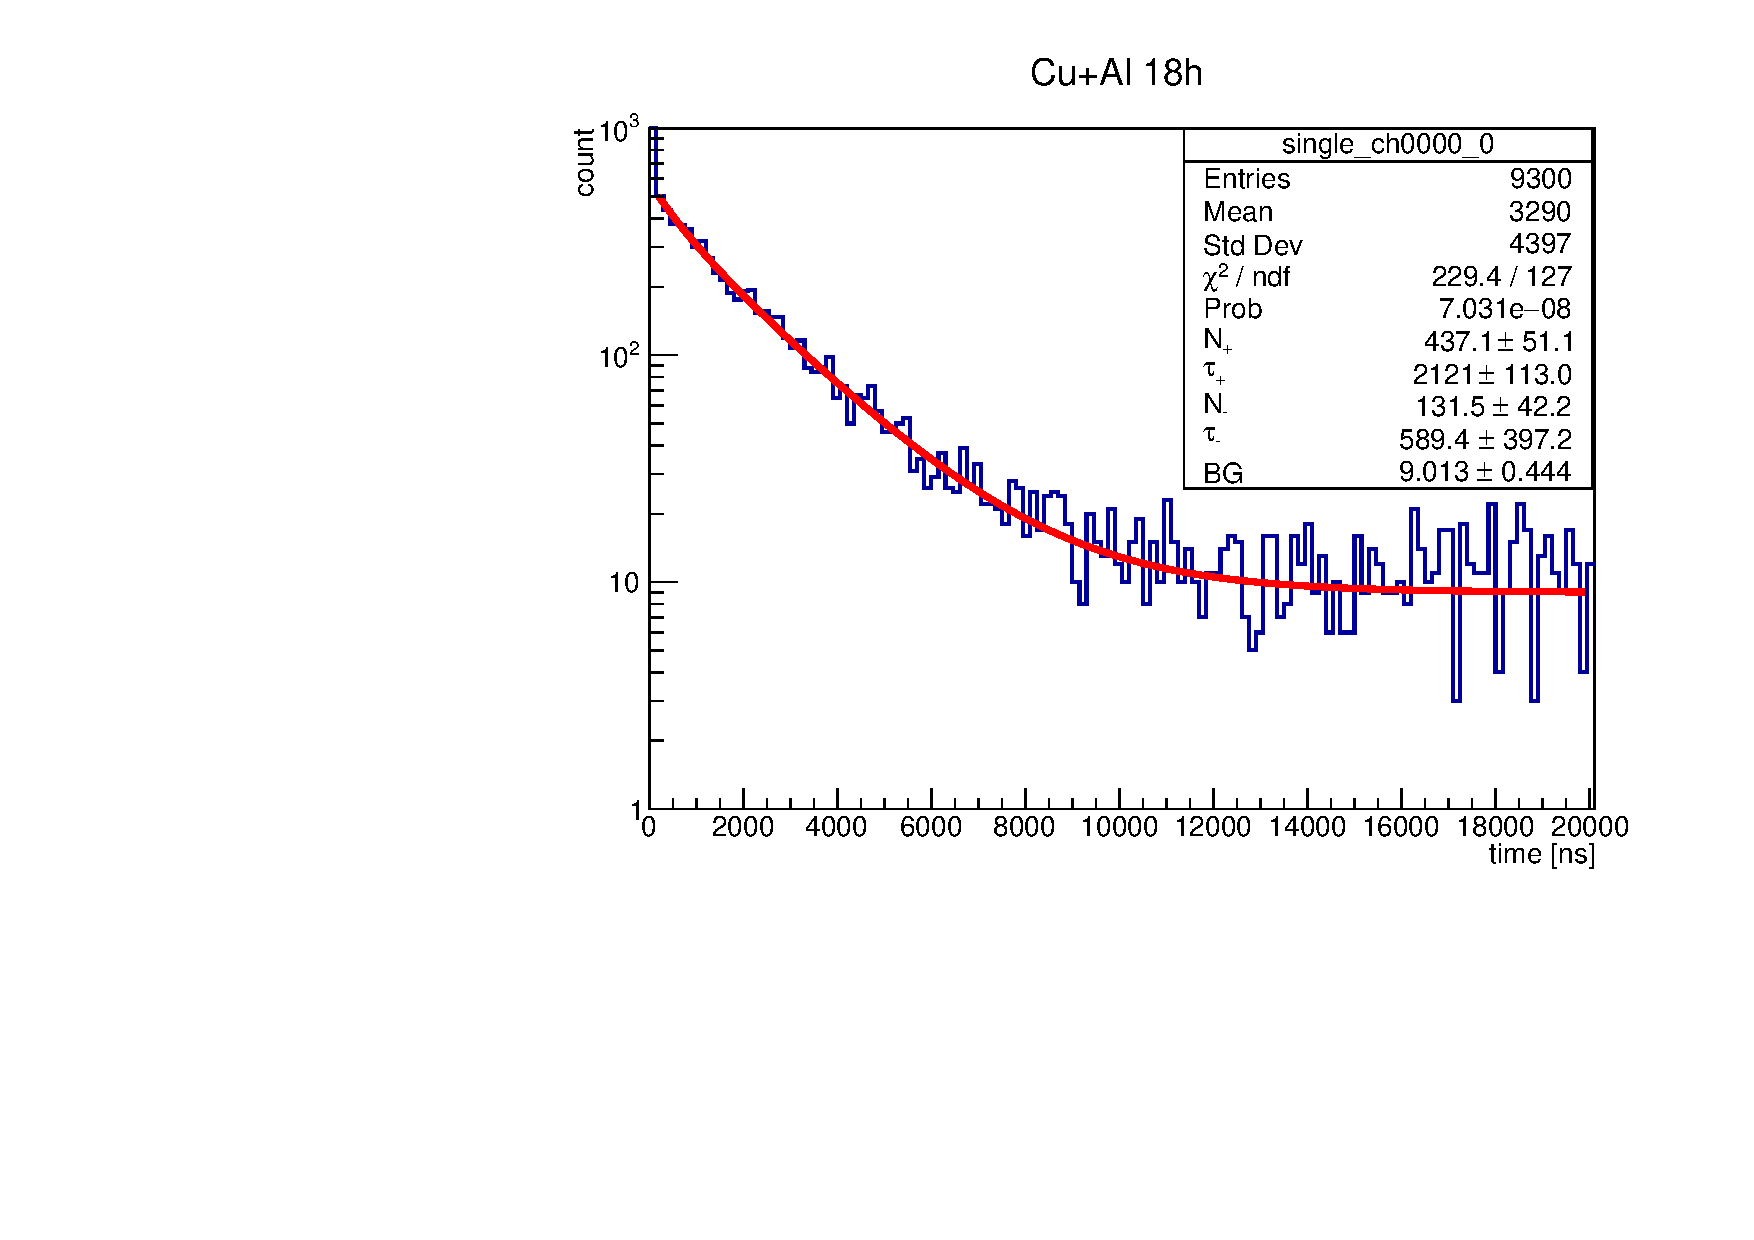
\includegraphics[width=7.5cm]{../img/results/CuAl18h.pdf}
            \subcaption{Cu, Al}
        \end{minipage}
        &
        \begin{minipage}[t]{0.5\hsize}
            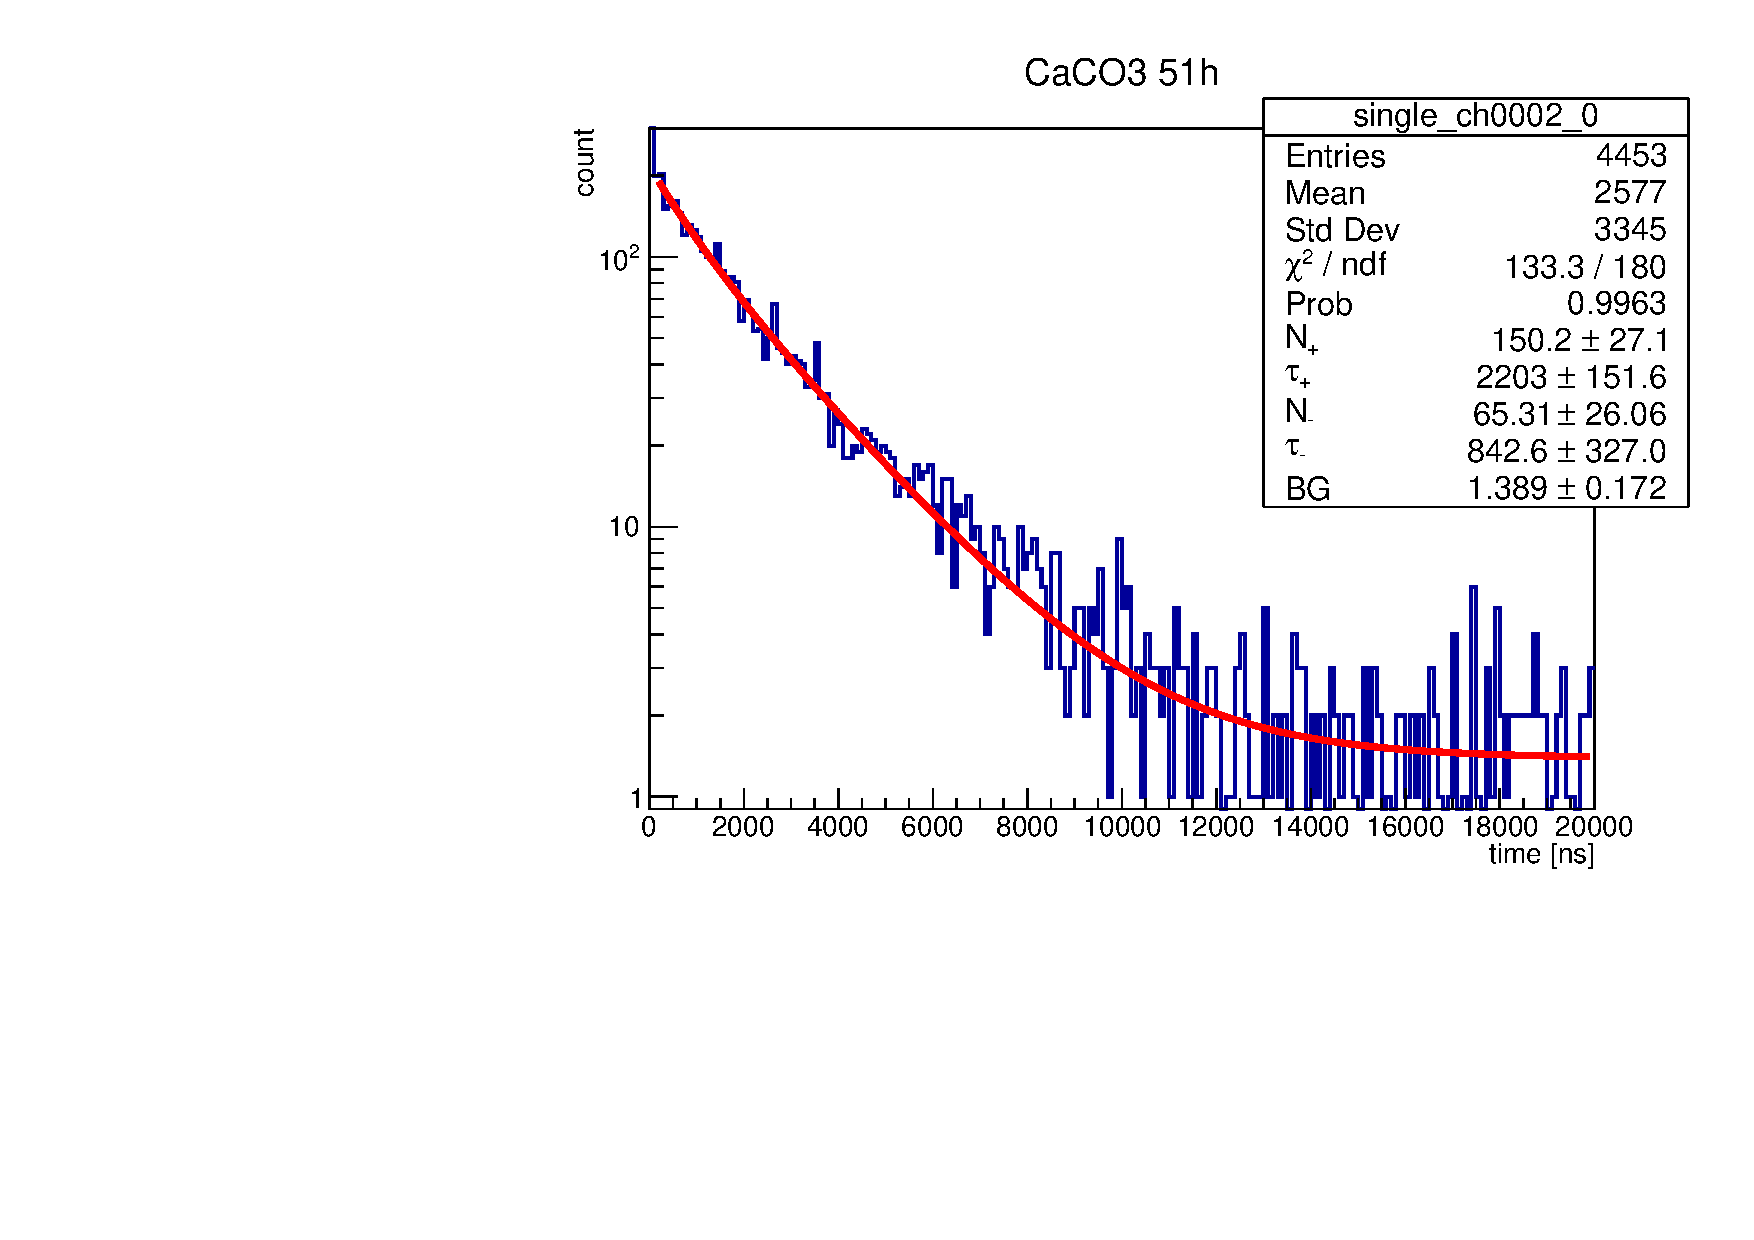
\includegraphics[width=7.5cm]{../img/results/CaCO3for51h.pdf}
            \subcaption{大理石}
        \end{minipage}
    \end{tabular}
    \caption{寿命測定結果}
    \label{fig: result: CaCO3}
\end{figure}

\begin{table}
    \centering
    \caption{$\mu^\pm$の寿命測定結果. 文献値は\cite{Ito Kaji Tabata Yoshiwara}から. }
    \begin{tabular}{llrr}
        \toprule
        試料 & 粒子 & 寿命$[\unit{\micro\second}]$ & 文献値$[\unit{\micro\second}]$
        \\
        \midrule
        Cu, Al & $\mu^+$ & $2.12\pm0.11$ & $2.20$
        \\
         & $\mu^-$ & $0.59\pm0.40$ & Cu: $0.16$, Al: $0.86$
        \\
        大理石 & $\mu^+$ & $2.20\pm0.15$ & $2.20$
        \\
         & $\mu^-$ & $0.84\pm0.33$ & Ca: $0.33$, C: $2.04$, O: $0.81$
        \\
        \bottomrule
    \end{tabular}
    \label{table: result: life}
\end{table}

特にCu, Alの結果についてはフィッティングの$\chi^2$値の上側累積確率が極端に小さく信頼性に乏しい.
大理石を試料としたものはその点問題ない.
特に$\mu^+$の結果は文献値によく沿っている.
また$\mu^-$については構成元素単体の寿命の中間をとることがわかる.
% 考察. 特に負ミュオンはもっと欲しい.

以上により, $\mu^+$の寿命及び$\mu^-$の原子核捕獲が計測された.


\subsection{スピン偏極}

測定結果に\eqref{eq: method: rough fitting of spin polarization by exp}でフィッティングしたものを図\ref{fig: exp fit of Larmor experiment}に掲げる.
磁場をかけることでカウントは\eqref{eq: N under Larmor}に従うはずであり\eqref{eq: method: rough fitting of spin polarization by exp}によるフィッティングは本来妥当でないが, この操作はバックグラウンドを差し引くためのものなので, $BG_U$の標準偏差及び$\chi^2$値の上側累積確率などフィッティングの信頼性は特に留意しない.
各変数は表\ref{table: result: parameters of result with B fit with exp}のようになる.

\begin{figure}
    \centering
    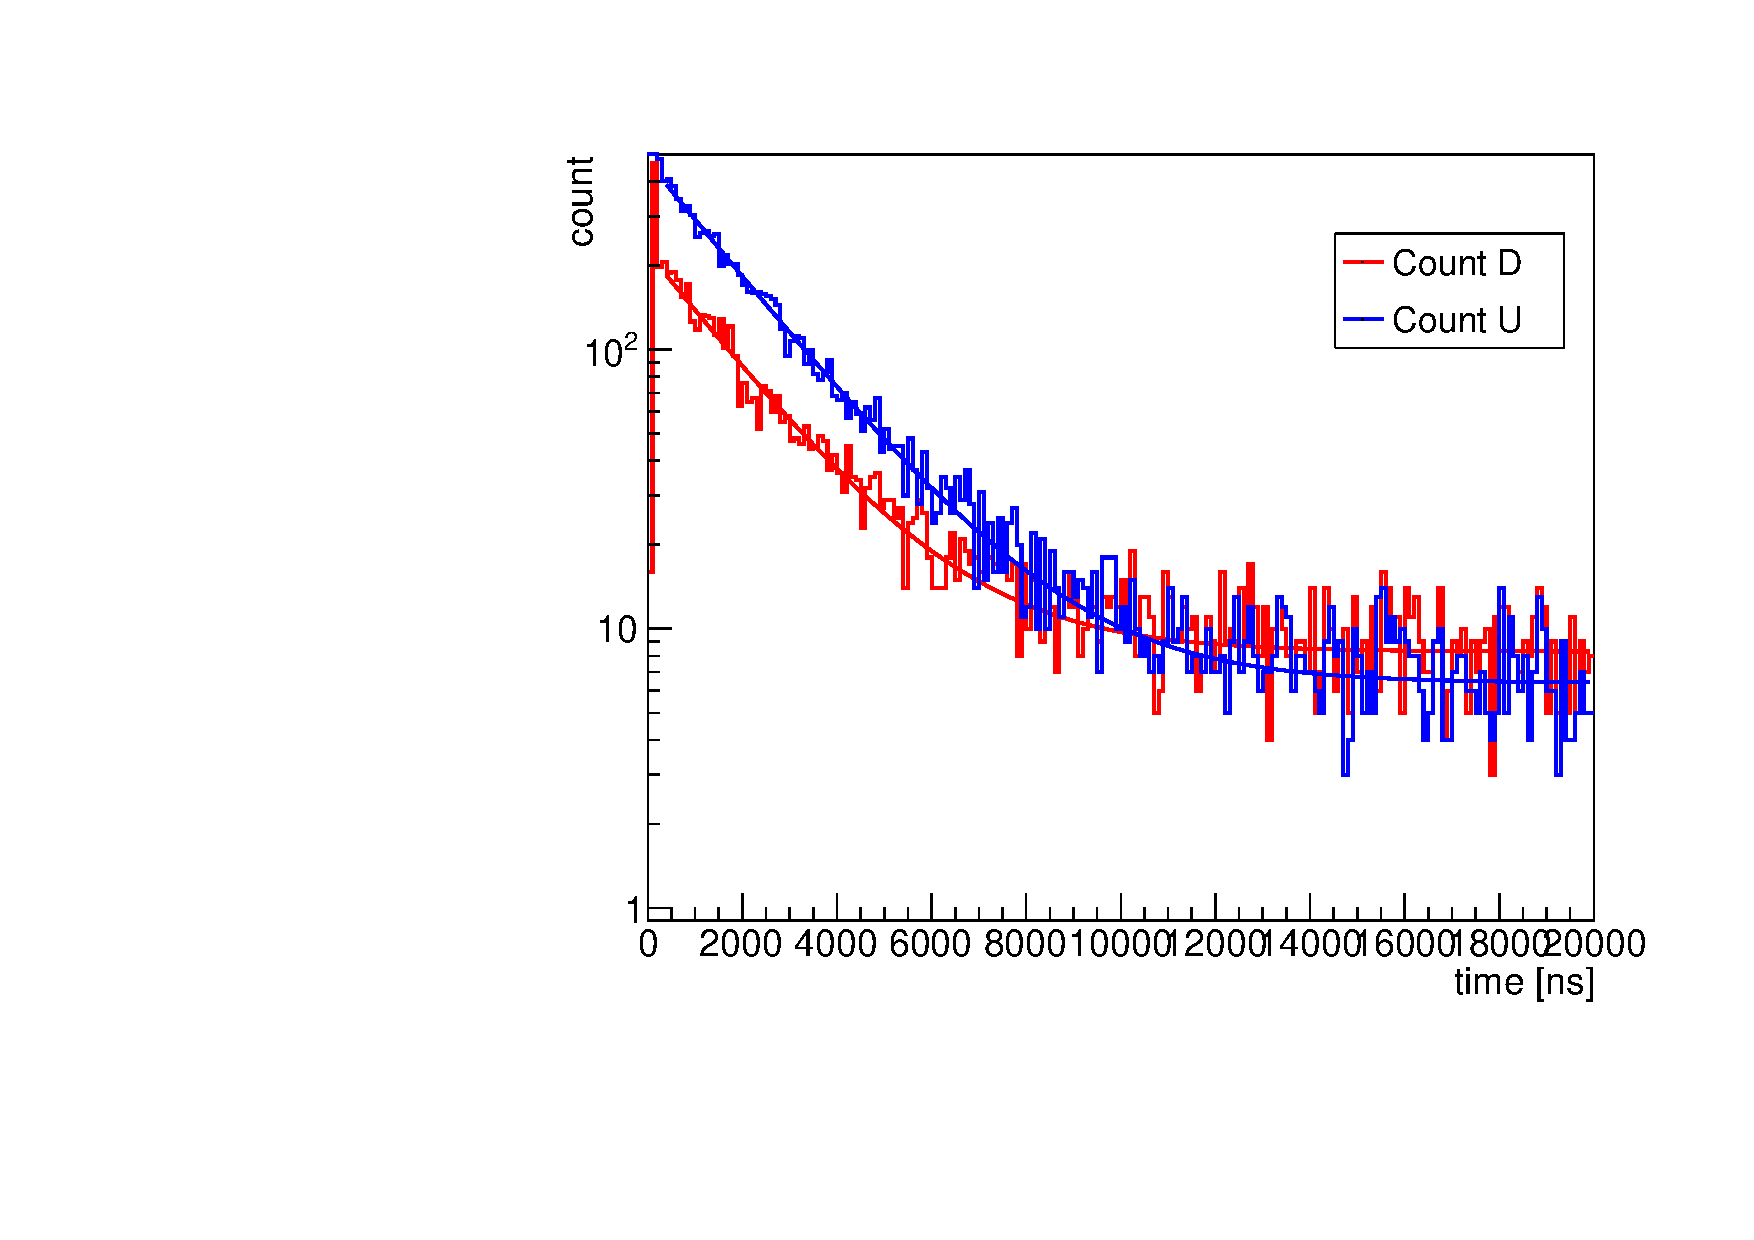
\includegraphics[width=8cm]{../img/results/expFit.pdf}
    \caption{スピン偏極測定で得られるデータと\eqref{fig: exp fit of Larmor experiment}によるフィッティング}
    \label{fig: exp fit of Larmor experiment}
\end{figure}

\begin{table}
    \centering
    \caption{\eqref{eq: method: rough fitting of spin polarization by exp}によってフィッティングしたときの変数値}
    \begin{tabular}[]{lrr}
        \toprule
        $N_U^0$ & $4.63817e+02\:\pm8.72257e+00$
        \\
        $\tau_U$ & $2.07050e+03\:\pm3.18642e+01$
        \\
        $BG_U$ & $6.39559e+00\:\pm2.74083e-01$
        \\
        \midrule
        $N_D^0$ & $2.14776e+02\:\pm6.68531e+00$
        \\
        $\tau_D$ & $2.00158e+03\:\pm5.62010e+01$
        \\
        $BG_D$ & $8.27831e+00\:\pm2.91137e-01$
        \\
        \bottomrule
    \end{tabular}
    \label{table: result: parameters of result with B fit with exp}
\end{table}

次いで$\alpha$を$0\leq\alpha\leq5$で$0.01$ずつ変えて非対称度\eqref{eq: method: fit asymmetry}を計算し, $A\cos(2\pi ft)$にフィッティングさせたときの$\chi^2$値を図\ref{fig: result: alpha and chi square}に示す.
極値は$(\alpha,\chi^2)=(2.23, 0.85)$であり, 上側累積確率は$74.7\%$である.
そこで$\alpha=2.23$を採用して\eqref{eq: method: fit asymmetry}を描き$\cos$でフィッティングすると図\ref{fig: result: asymmetry}の通りになる.

\begin{figure}
    \centering
    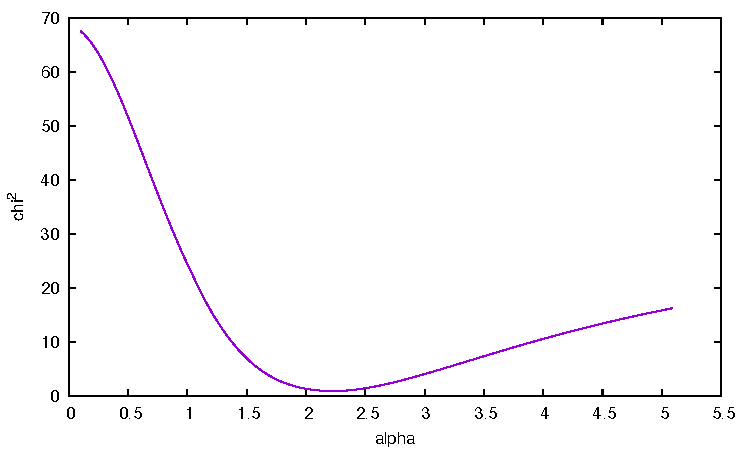
\includegraphics[width=8cm]{../img/results/alpha-chi2.pdf}
    \caption{$\alpha$を変えて非対称度\eqref{eq: method: fit asymmetry}を三角関数でフィッティングしたときの$\chi^2$値}
    \label{fig: result: alpha and chi square}
\end{figure}

\begin{figure}
    \centering
    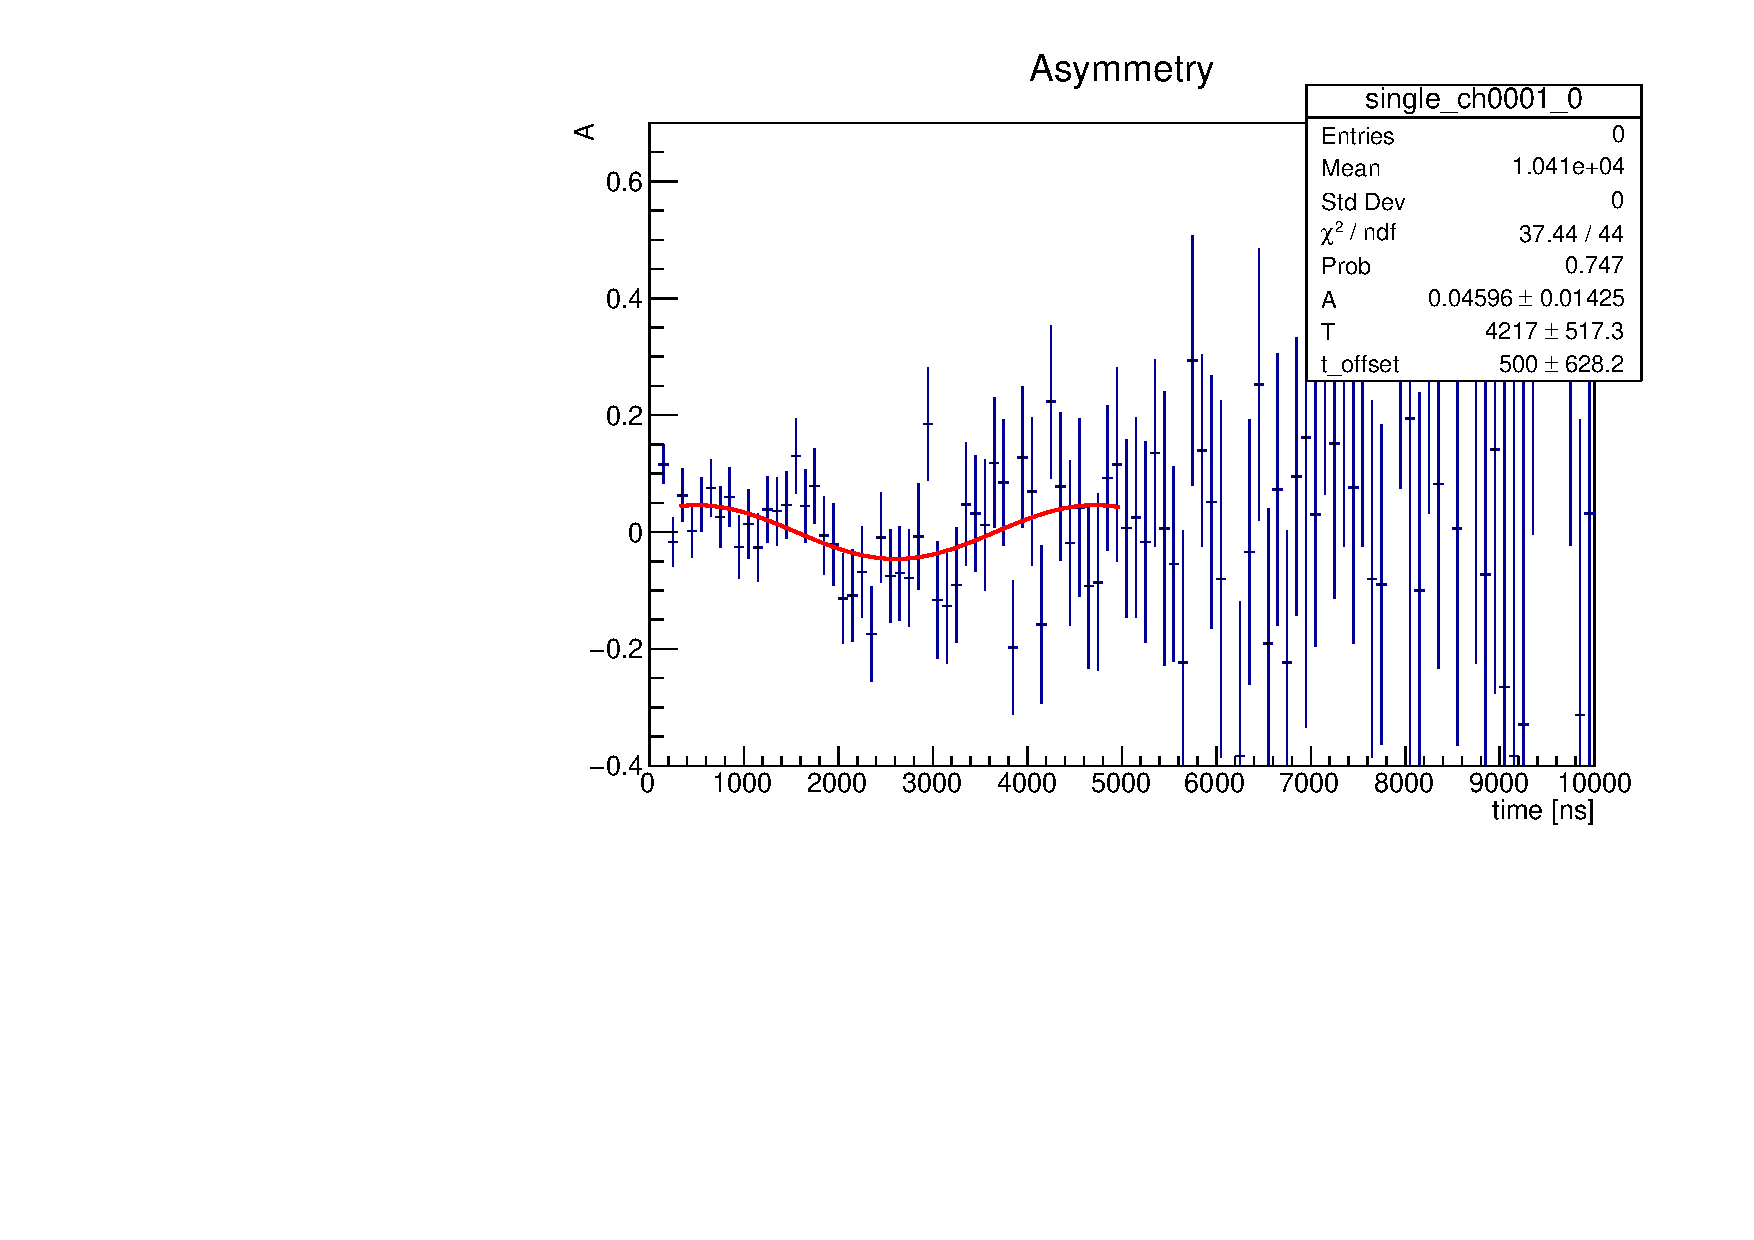
\includegraphics[width=9cm]{../img/results/asymmetry.pdf}
    \caption{非対称度$\mathscr{A}$と$\cos$によるフィッティング}
    \label{fig: result: asymmetry}
\end{figure}

これより振動周期$T=\SI{4.217\pm0.517}{\second}$を得て, \eqref{eq: Larmor precession}より磁場を計算すると$B=\SI{1.75+-0.22}{\milli\tesla}$となる.
$B_{\text{design}}=\SI{2}{\milli\tesla}$と比較して, この結果が妥当であることが確かめられる.

以上より, ミュオンのスピンが運動量に応じて偏極していることが確認された.


\appendix


\section{論理回路}
\label{sec: logic circuit}

実験で実際に用いたNIMモジュールの回路を図\ref{fig: full circuit}に掲げる.
主にCu, Alからの信号の入力部(Cu, Al), 大理石からの入力部($\mathrm{CaCO_3}$), 制御部(GATES), 出力部(OUTPUTS)に大別できる.

入力はTUD各層それぞれ3組のPSc+PMTから引いている.
粒子のカウント数が各PScにてミュオンの飛来数に合わせ$\SI{1}{count/\cm^2/\min}$となるように閾値を設定しておく\cite{Grupen}.
% 文献ほしい
それぞれT1, T2, T3, U1, ...と番号を振っている.
Cu, AlのTに描いたようなor接続をCu, AlのU以下全ての入力端子でとっているが, 簡単のためCu, AlのT以外は省略した.
なお, このor接続以前でdelayを置いているのはCu, AlのTのみである.

制御部GATESはCu, Alと大理石の信号が干渉しないようにスイッチの役割を果たす.
具体的には, Cu, Al側のGGが起動している間は大理石の信号が入ってもstopと判定しない.
逆もまた然りである.

DAQ-PCでは短時間に複数のstart信号を受けたとき最初の信号のみを使用し, それ以降の信号は停止信号を得るか所定の時間($\SI{20}{\micro\second}$)無視する.

\begin{landscape}
    \begin{figure}
        \centering
        % displaying the circuit without rotation
\begin{circuitikz}
    % B
    \draw
        (1,0)
        % TUnotD
        node[ieeestd and port, number inputs=3, anchor=in 1] (BTUnotD) {}
        % T
        (BTUnotD.in 1) to[short] ++(-1,0)
        node[anchor=east](BT){$\mathrm{CaCO_3}$ T}
        % gateBlocal
        (BTUnotD.out) to[short] ++(0.5,0)
        node[twoportshape, anchor=west, t=GG] (gateBlocal){} ++(1,0)
        % gate delay
        to [short] ++(0.5,0)
        node[align=left, anchor=west](gateBdelay){\small delay\\$\SI{31}{\nano\second}$} ++(1,0)
        % to D stop
        to [short] ++(0.5,0)
        to [short, *-] ++(0,-1.5)
        to [short] ++(0.55,0)
        node[ieeestd and port, anchor=in 1] (BDstoplocal){}
        % (BDstoplocal.out) node[anchor=west]{D stop}
        ;
        % not D
        \node
        at (BTUnotD.bin 3) [ocirc, left]{}
        ;
        % gateBdelay to U stop
        \draw
        (gateBdelay.east)
        to [short] ++(1,0)
        node[ieeestd and port, anchor=in 1](BUstoplocal){} ++(1,0)
        % (BUstoplocal.out) node[anchor=west]{U stop}
        ;
        % start
        \draw
        (BTUnotD.out) to[short, *-] ++(0,1)
        to[short] ++(3.5,0)
        node[anchor=west](Bstart){}
        ;
        \draw
        (BTUnotD.in 2) to[short] ++(-1,0)
        node[anchor=east](U){$\mathrm{CaCO_3}$ U}
        (BTUnotD.in 3) to[short] ++(-1,0)
        node[anchor=east](D){$\mathrm{CaCO_3}$ D}
        (0.5,-0.38) to [short, *-] ++(0,-1)
        -- ++(2,0)
        node[align=left, anchor=west]{\small delay\\ $\SI{2}{\nano\second}$} ++(1,0)
        -| (BUstoplocal.in 2)
        (0.7, -0.75) to [short, *-] ++(0,-1.4)
        |- (BDstoplocal.in 2)
        % node [anchor=north](Ddelay){delay}
        % (Ddelay.east) -- (BDstoplocal.in 2)
        % U stop
        (15,-0.3) node[ieeestd and port, anchor=center, number inputs=3](BUstop){}
        (BUstop.out) node[anchor=west]{$\mathrm{CaCO_3}$ U stop}
        % D stop
        (15,-1.8) node[ieeestd and port, anchor=center, number inputs=3](BDstop){}
        (BDstop.out) node[anchor=west](BDstopLabel){$\mathrm{CaCO_3}$ D stop}
        (BUstoplocal.out) -- (BUstop.in 3)
        (BDstoplocal.out) -- (BDstop.in 3)
        ;
        % box
        \node[rectangle,draw,dashed,fit=(BT) (BDstoplocal) (BDstoplocal)](CaCO3){};
        \node[anchor=north, align=center] at (CaCO3.south){$\mathrm{CaCO_3\:INPUTS}$};
    % A
    \draw
        % T
        (2,6)
        node[ieeestd or port, number inputs=3, anchor=in 1] (ATor) {}
        % T1E
        (0,7) node[anchor=east](T1E){Cu, Al T1}
        -- ++(1.2,0)
        node[align=left, anchor=west](T1Edelay){\small delay\\ $\SI{22}{\nano\second}$} (1,0)
        (T1Edelay.south) |- (ATor.in 1)
        % T2E
        (0,5.62)
        node[anchor=east]{Cu, Al T2}
        -- ++(0.5,0)
        node[align=left, anchor=west](T2Edelay){\small delay\\ $\SI{14}{\nano\second}$} (1,0)
        (T2Edelay.east) -- (ATor.in 2)
        % T3E
        (0,4.5)
        node[anchor=east]{Cu, Al T3}
        -- ++(1.2,0)
        node[align=left, anchor=west](T3Edelay){\small delay\\ $\SI{30}{\nano\second}$}
        (T3Edelay.north) |- (ATor.in 3)
        ;
        \draw
        % TUnotD
        (4.5,3.625)
        node[ieeestd and port, number inputs=3, anchor=in 1](ATUnotD){}
        (ATor.out) |- (ATUnotD.in 1)
        % U
        (ATUnotD.in 2)
        to[short] (0,3.25)
        node[anchor=east]{Cu, Al U}
        % D
        (ATUnotD.in 3)
        to[short] (0,2.9)
        node[anchor=east](AD){Cu, Al D}
        ;
        % not D
        \node at (ATUnotD.bin 3) [ocirc, left]{};
        % AU stop
        \draw
        (15,8) node[ieeestd and port, anchor=center, number inputs=3](AUstop){}
        ;
        \draw
        % U to Ustop
        (3,3.25)
        to [short, *-] ++(0,1.5)
        -| ++(2,3.6)
        -- ++(1,0)
        node[anchor=west, align=left]{\small delay\\ $\SI{30}{\nano\second}$} ++(1,0)
        % to [short] ++(1,0)
        -- (AUstop.in 1)
        % AD stop
        (15,6.5) node[ieeestd and port, anchor=center, number inputs=3](ADstop){}
        ;
        % D to Dstop
        \draw
        (3.5,2.9)
        to [short, *-] ++(0,1.2)
        -| ++(2,3.2)
        to [short] ++(1,0)
        -| (ADstop.in 1)
        (AUstop.out) node[anchor=west](AUstopLabel){Cu, Al U stop}
        (ADstop.out) node[anchor=west]{Cu, Al D stop}
        ;
        % box
        \node[rectangle,draw,dashed,fit=(T1E) (AD) (ATUnotD) (T1Edelay)](CuAl){};
        \node[anchor=north, align=center] at (CuAl.south){Cu, Al INPUTS};
    % gate
    \draw
        % and9
        (10,2.97)
        node[ieeestd and port, anchor=center](and9){}
        % and10
        (10,5)
        node[ieeestd and port, anchor=center](and10){}
        % ATUnotD to 9
        (ATUnotD.out) |- (and9.in 1)
        % gateA
        (8.2,6.5) node[twoportshape, anchor=center, t=GG](gateA){}
        % gateB
        (8.2,1) node[twoportshape, anchor=center, t=GG](gateB){}
        (Bstart.west) |- (and10.in 2)
        % start trigger
        (15,4)
        node[ieeestd or port, anchor=center](STARTor){}
        (STARTor.out) node[anchor=west]{start}
        % 9 and 10 to start or
        (and9.out) |- (STARTor.in 2)
        (and10.out) |- (STARTor.in 1)
        % 9 to gate A
        (and9.out) to [short, *-] ++(0,-1)
        to [short] ++(-4,0)
        |- (gateA.west)
        % 10 to gate B
        (and10.out) to [short, *-] ++(0,0.9)
        to [short] ++(-3.7,0)
        |- (gateB.west)
        ;
        \draw
        % gate B to BU stop
        (gateB.east) to[short, -*] (13,1)
        |- (BDstop.in 2)
        % gate B to BD stop
        (13,-0.3) to[short, *-] (BUstop.in 2)
        % gate B to A stop
        (gateB.east) -- (13,1)
        |- (AUstop.in 3)
        (13,6.13) to[short, *-] (ADstop.in 3)
        ;
        \node
        at (AUstop.bin 3) [ocirc, left]{}
        ;
        \node
        at (ADstop.bin 3) [ocirc, left]{}
        ;
        % gate B to 9
        \draw
        (gateB.east) to[short] ++(0.2,0)
        to [short, *-] ++(0,0.2)
        |- (and9.in 2)
        ;
        \node
        at (and9.bin 2) [ocirc, left]{}
        ;
        % gate A to 10
        \draw
        (gateA.east) to[short] ++(0.2,0)
        to [short, *-] ++(0,-0.2)
        |- (and10.in 1)
        ;
        \node
        at (and10.bin 1) [ocirc, left]{}
        ;
        \draw
        % gate A to A stop
        (12,6.5) to[short, *-] ++(0,1.5)
        -- (AUstop.in 2)
        (12,6.5) -- (ADstop.in 2)
        % gate A to B stop
        (gateA.east) to[short] (12,6.5)
        |- (BDstop.in 1)
        ;
        \node
        at (BDstop.bin 1) [ocirc, left]{}
        ;
        \draw
        (12,0.06) to[short, *-] (BUstop.in 1)
        ;
        \node
        at (BUstop.bin 1) [ocirc, left]{}
        ;
        % box
        \node[rectangle,draw,dashed,fit=(gateA) (gateB) (and9) (and10)](gates){};
        \node[anchor=north east, align=left] at (gates.south east){GATES};
    % outputs box
    \node[rectangle,draw,dashed,fit=(AUstop)(BDstop)(AUstopLabel)(BDstopLabel)](outputs){};
    \node[anchor=north, align=center]at(outputs.south){OUTPUTS};
\end{circuitikz}

        \caption{実験で用いた論理回路}
        \label{fig: full circuit}
    \end{figure}
\end{landscape}


% \section{解析コード}

% ここでは解析に用いたコードの概要を示す.
% 変数の宣言やヒストグラムの取得などは省略しているため, 表示の通りに実装しても作動しない.
% 実際に解析で使用したものは\url{https://github.com/LowToneVoice/ksc16/tree/main/group7/analysis}を参照のこと.
% また測定データを\url{https://github.com/LowToneVoice/ksc16/tree/main/group7/data}に置いている.
% 置いとくならこのセクションいらない?

% \subsection{寿命測定}

% \begin{mylisting}[language=c++, caption=addfitCuAl.C]
% void addfitCuAl()
% {
%     // sum of hists
%     hu->Add(hd, 1);
%     // configure bin of hist
%     hu->Rebin(50);

%     // fitting curve
%     TF1 *f1 = new TF1("f1", "[ 0 ] * exp( -x / [ 1 ]) + [ 2 ] * exp( -(x + [ 3 ]) / [ 4 ]) +  [ 5 ] ");
%     f1->SetParameters(100, 2200.0, 100, 0, 2100.0, 0.0);
%     f1->SetParNames("N_{+}", "#tau_{+}", "N_{-}", "td_0", "#tau_{-}", "BG");
%     hu->Fit("f1", "", "", 100, 20000);

%     // y axis to log scale
%     c1->SetLogy();
%     hu->Draw();
% }
% \end{mylisting}

% \begin{mylisting}[language=c++, caption=addfitCa.C]
% void addfitCa()
% {
%     // sum of hists
%     hu->Add(hd);
%     // configure bin of hist
%     hu->Rebin(100);
%     hu->Draw();

%     // fitting curve
%     TF1 *f1 = new TF1("f1", "[ 0 ] * exp( -(x / [ 1 ])) + [ 2 ] * exp( -(x / [ 3 ])) +  [ 4 ] ");
%     f1->SetParameters(150, 2000.0, 120, 900.0, 2.0);
%     f1->SetParNames("N_{+}", "#tau_{+}", "N_{-}", "#tau_{-}", "BG");
%     hu->Fit("f1", "", "", 100, 20000);
%     // y axis to log scale
%     c1->SetLogy();
% }
% \end{mylisting}

% \subsection{スピン偏極測定}

% 各コードで何が出てくるか, どうやって運用するかを記述.
% まずexpFit.Cで\eqref{eq: method: rough fitting of spin polarization by exp}のフィッティングを行いバックグラウンドを求める.
% \eqref{eq: method: fit asymmetry}の$\cos$によるフィッティングの$\chi^2$値を複数の$\alpha$で計算する.
% $\chi^2$が極小となる$\alpha$を選び\eqref{eq: method: fit asymmetry}のフィッティングパラメーターを結果とする.

% \begin{mylisting}[language=c++,caption=expFit.C]
% void expFit()
% {
%     // configure bin of hist
%     hu->Rebin(100);
%     hd->Rebin(100);

%     // fitting curve
%     TF1 *fu = new TF1("fu", "[0] * exp(-x / [1]) + [2]");
%     TF1 *fd = new TF1("fd", "[0] * exp(-x / [1]) + [2]");
%     fu->SetParameters(200.0, 2000.0, 0.0);
%     fu->SetParNames("N_U", "#tau_U", "BG_U");
%     fd->SetParameters(100.0, 2000.0, 0.0);
%     fd->SetParNames("N_D", "#tau_D", "BG_D");
%     hu->Fit("fu", "", "", 300, 20000);
%     hd->Fit("fd", "", "", 300, 20000);

%     hd->Draw();
%     hu->Draw("same");
%     // y axis to log scale
%     c1->SetLogy();
% }
% \end{mylisting}

% \begin{mylisting}[language=c++,caption=findPar.C]
% void findPar()
% {
%     // hists
%     h1_init = (TH1D *)h1->Clone();
%     h2_init = (TH1D *)h2->Clone();

%     for (i = 0; i < 500; i++)
%     {
%         offset = -30;
%         alpha = 0.1 + i * 0.01;

%         h1 = (TH1D *)h1_init->Clone();
%         h2 = (TH1D *)h2_init->Clone();

%         // move h2 left for offset
%         for (k = 0; k < h2->GetXaxis()->GetNbins(); k++)
%         {
%             if (offset + k < 0)
%             {
%                 h2->SetBinContent(k, 0);
%             }
%             else
%             {
%                 h2->SetBinContent(k, h2_init->GetBinContent(k + offset));
%             }
%         }

%         // rebin
%         h1->Rebin(100);
%         h2->Rebin(100);

%         // for error evaluation
%         h1->Sumw2();
%         h2->Sumw2();

%         // delete BGs
%         for (k = 0; k < h1->GetXaxis()->GetNbins(); k++)
%         {
%             h1->SetBinContent(k, h1->GetBinContent(k) - bg_u);
%         }
%         for (k = 0; k < h2->GetXaxis()->GetNbins(); k++)
%         {
%             h2->SetBinContent(k, h2->GetBinContent(k) - bg_d);
%         }
%         h3 = (TH1D *)h1->Clone();
%         h4 = (TH1D *)h2->Clone();

%         // h2 times alpha
%         for (k = 0; k < h2->GetXaxis()->GetNbins(); k++)
%         {
%             h2->SetBinContent(k,  (h4->GetBinContent(k) * alpha));
%             h2->SetBinError(k, (h4->GetBinError(k) * alpha));
%         }

%         // D-U/D+U
%         h3 = (TH1D *)h1->Clone();
%         h4 = (TH1D *)h2->Clone();
%         h4->Add(h3, -1);
%         h2->Add(h1);
%         h4->Divide(h2);

%         // fitting by cos
%         TF1 *f = new TF1("f", "[0] * cos(2 * TMath::Pi() * (x - [2]) / [1])");
%         f->SetParNames("A", "T", "t_offset");
%         f->SetParameters(.1, 3500, .0);
%         f->SetParLimits(0, .01, .5);
%         f->SetParLimits(1, 2500, 4500);
%         f->SetParLimits(2, -500., 500.);
%         h4->Fit("f", "", "", 300, 5000);

%         // output chi^2/ndf and prob
%         erfun = h4->GetFunction("f")->GetChisquare();
%         ndf = h4->GetFunction("f")->GetNDF();
%         prob = h4->GetFunction("f")->GetProb();
%         outputfile_chi2 << alpha << " " << erfun / ndf << " ";
%         outputfile_prob << alpha << " " << prob << " ";

%         // change the lines of
%         outputfile_chi2 << endl;
%         outputfile_prob << endl;
%     }
%     outputfile_chi2.close();
%     outputfile_prob.close();
% }
% \end{mylisting}

% \begin{mylisting}[language=c++,caption=fitAsym.C]
% void fitAsym()
% {
%     offset = -30;
%     alpha = 2.23;
%     // hists
%     h1_init = (TH1D *)h1->Clone();
%     h2_init = (TH1D *)h2->Clone();

%     // move h2 left for offset
%     for (i = 0; i < h2->GetXaxis()->GetNbins(); i++)
%     {
%         if (offset + i < 0)
%         {
%             h2->SetBinContent(i, 0);
%         }
%         else
%         {
%             h2->SetBinContent(i, h2_init->GetBinContent(i + offset));
%         }
%     }

%     // rebin
%     h1->Rebin(100);
%     h2->Rebin(100);

%     // for error evaluation
%     h1->Sumw2();
%     h2->Sumw2();

%     // delete BGs
%     for (i = 0; i < h1->GetXaxis()->GetNbins(); i++)
%     {
%         h1->SetBinContent(i, h1->GetBinContent(i) - bg_u);
%     }
%     for (i = 0; i < h2->GetXaxis()->GetNbins(); i++)
%     {
%         h2->SetBinContent(i, h2->GetBinContent(i) - bg_d);
%     }
%     h3 = (TH1D *)h1->Clone();
%     h4 = (TH1D *)h2->Clone();

%     // h2 times alpha
%     for (i = 0; i < h2->GetXaxis()->GetNbins(); i++)
%     {
%         h2->SetBinContent(i, h4->GetBinContent(i) * alpha);
%         h2->SetBinError(i, h4->GetBinError(i) * alpha);
%     }

%     // D-U/D+U
%     h3 = (TH1D *)h1->Clone();
%     h4 = (TH1D *)h2->Clone();
%     h4->Add(h3, -1);
%     h2->Add(h1);
%     h4->Divide(h2);

%     // fitting by cos
%     TF1 *f = new TF1("f", "[0] * cos(2 * TMath::Pi() * (x - [2]) / [1])");
%     f->SetParNames("A", "T", "t_offset");
%     f->SetParameters(.1, 3500, .0);
%     f->SetParLimits(0, .01, .5);
%     f->SetParLimits(1, 2500, 4500);
%     f->SetParLimits(2, -500., 500.);
%     h4->Fit("f", "", "", 300, 5000);

%     h4->Draw();
% }
% \end{mylisting}



\begin{thebibliography}{10}
    \bibitem{Grupen} Claus Grupen, 小早川惠三訳「宇宙素粒子物理学」シュプリンガー・ジャパン(2009)
    \bibitem{PDG} M. Tanabashi \textit{et al.} (Particle Data Group), Phys. Rev. D \textbf{98}, 030001 (2018)
    % \bibitem{Sakai} 坂井典佑「物理学基礎シリーズ10 素粒子物理学」培風館(1996)
    % \bibitem{KEK} 門野良典, 足立伸一, 小野寛太, 稲田康宏, 伊藤晋一, 鬼柳善明, 大友季哉, 兵頭俊夫「KEK物理学シリーズ第6巻 量子ビーム物質科学」共立出版(2013)
    \bibitem{Ito Kaji Tabata Yoshiwara} 伊藤泰男,鍛冶東海,田畑米穂,吉原賢二,「素粒子の化学」学会出版センター(1985)
\end{thebibliography}
\end{document}
